\documentclass[11pt]{article}

\usepackage[a4paper, margin=1in]{geometry}
\usepackage{mathtools}
\usepackage{outlines}
\usepackage{amsmath}
\usepackage{pdfpages}
\usepackage{verbatim}
\usepackage{listings}
\usepackage{algorithm}
\usepackage[noend]{algpseudocode}
% \usepackage[dvipsnames]{xcolor}
\usepackage[english]{babel}
\usepackage[labelfont=bf]{caption}
\usepackage{hyperref}
\usepackage{subcaption}
\usepackage{array}
\usepackage{longtable}
%\usepackage[T1]{fontenc}
\usepackage{titlesec, blindtext, color}
\usepackage{float}
\usepackage{graphicx}
\usepackage{xcolor}
\usepackage{dirtree}
\usepackage{pythonhighlight}
\pagecolor{white}
\definecolor{gray75}{gray}{0.75}
\newcommand{\hsp}{\hspace{10pt}}
\titleformat{\section}[hang]{\Huge\bfseries}{\thesection\hsp\textcolor{gray75}{|}\hsp}{0pt}{\Huge\bfseries}

\captionsetup{labelfont=bf}

\makeatletter
\def\BState{\State\hskip-\ALG@thistlm}
\makeatother

\definecolor{codegreen}{rgb}{0,0.6,0}
\definecolor{codegray}{rgb}{0.5,0.5,0.5}
\definecolor{codepurple}{rgb}{0.58,0,0.82}
\definecolor{backcolour}{rgb}{0.95,0.95,0.95}


\lstdefinestyle{mystyle}{
    backgroundcolor=\color{backcolour},   
    commentstyle=\color{codegreen},
    keywordstyle=\color{blue},
    numberstyle=\tiny\color{codegray},
    stringstyle=\color{orange},
    basicstyle=\ttfamily\footnotesize,
    breakatwhitespace=false,         
    breaklines=true,                 
    captionpos=b,                    
    keepspaces=true,                 
    numbers=left,                    
    numbersep=5pt,                  
    showspaces=false,                
    showstringspaces=false,
    showtabs=false,                  
    tabsize=2
}

\lstset{style=mystyle}

\includeonly{
    chapters/introduction,
    chapters/geninfo,
    chapters/scratch,
    chapters/pretrained,
    chapters/baseline,
    chapters/ensemble
}


\begin{document}
\begin{titlepage}
    \begin{center}
        \begin{figure}
            
\includegraphics[width=\textwidth]{img/marchio_unipi_pant541-eps-converted-to.pdf}         
        \end{figure}
        {\Large
        Artificial Intelligence and Data Engineering\\
        \vspace{5mm} %5mm vertical space
        Computational Intelligence and Deep Learning}\\
        \vspace{30mm} %5mm vertical space
        {\Huge\textbf{\textit{Artist Identification with Convolutional Neural Networks}}}\\
        \vspace{10mm} %5mm vertical space
        {\Large Project Documentation}\\
        \par\noindent\rule{\textwidth}{0.4pt}
            \begin{flushright}
                \textit{TEAM MEMBERS}:\\
                Edoardo Fazzari\\ 
                Mirco Ramo\\
        	
            \end{flushright}
            \vfill
        Academic Year: 2020/2021\\        
    \end{center}
\end{titlepage} 
   
\tableofcontents

\section{Introduction}
Artist identification is traditionally performed by \textit{art historians} and \textit{curators} who have expertise and familiarity with different artists and styles of art. This is a complex and interesting problem for computers because identifying an artist does not just require object or face detection; artists can paint a wide variety of objects and scenes. Additionally, many artists from the same time period will have similar styles, and some such as \textbf{Pablo Picasso} (see figure \ref{fig:picasso}) have painted in multiple styles and changed their style over time.

de

\noindent The aim of this project is to use Convolutional Neural Networks for the identification of an artist given a painting. In particular, the CNN networks will be modeled using multiple techniques: from scratch; via pretrained network; networks based on comparison with baseline input and using an ensemble network made of by the best classifiers found.


\subsection{State of the Art}
As mentioned, artist identification has primarily been tackled by humans. An example of that is the Artsy's Art Genome Project \footnote{https://www.artsy.net/categories}, which is led by experts who manually classify art. This strategy is not very scalable even if it is highly precise in the classification (the site is a marketplace of fine-arts for collects, you can find Pisarro, Bansky and other famous artists).

Most prior attempts to apply machine learning to this problem have been feature-based, aiming to identify what qualities most effectively distinguish artists and styles. Many generic image features have been used, including scale-invariant feature transforms (SIFT), histograms of oriented gradients (HOG), and more, but with the focus on \textit{discriminating different style} in Fine-Art Painting\footnote{T. E. Lombardi. The classification of style in fine-art paint-
ing. ETD Collection for Pace University, 2005}.

The first time the problem of artist identification was really tackled was with J. Jou and S. Agrawal\footnote{J. Jou and S. Agrawal. Artist identification for renaissance paintings.} in 2011, they applied several multi-class classification techniques like Naïve Bayes, Linear Discriminant Analysis, Logistic Regression, K-Means and SVMs and achieve a maximum classification accuracy of 65\% for an unknown painting across 5 artists. 
Later on, the problem of identifying artists was retackled by the \textit{Rijksmuseum Challenge}\footnote{T. Mensink and J. van Gemert. The rijksmuseum challenge: Museum-centered visual recognition. 2014}. The objective of the challenge was to predict the artist, type, material and creation year (each of them was a different challenge) of the 112,039 photographic \footnote{The dataset contains 6,629 artists in total, with high variation in the number of pieces per artist. For example, Rembrandt has 1,384 pieces, and Vermeer has only 4. There are 350 artists with more than 50 pieces, 180 artists have around 100, and 90 artists have 200 pieces.} (containing different viewpoints of an artwork, and different types of them: sculptures, paintings, saucers, etc.) reproductions of the artworks exhibited in the Rijksmuseum in Amsterdam (the Netherlands). For the artist classification challenge, the paper said they read a test accuracy of about 60\%. The year later, Saleh and Elgammal's paper\footnote{B. Saleh and A. M. Elgammal. Large-scale classification of fine-art paintings: Learning the right metric on the right
feature. CoRR, abs/1505.00855, 2015} was the first attempt to identify artists with a large and varied dataset, but still using generic features. The collection they used has images of 81,449 fine-art paintings from 1,119 artists ranging from fifteen centuries to contemporary artists, reaching an accuracy of 59\%\footnote{In the paper they tried to use also CNN, but reaching only an accuracy of 33.62\%}.


More recent attempts are related to the \textit{Painter by Numbers}, a \textbf{Playground Prediction Competition} by \textit{Kaggle}\footnote{https://www.kaggle.com/c/painter-by-numbers/data}. This competition used a pairwise comparison scheme: participants had to create an algorithm which needs to examine two images and predict whether the two images are by the same artist or not. Thus, it is not our same objective, however it can be consider the first application of Deep Learning to the problem. The real deal was taken by Nitin Viswanathan\footnote{Nitin Viswanathan, Artist Identification with Convolutional Neural Networks} in 2017.
Viswanathan, using the same dataset of the mentioned \textit{Kaggle Challenge}, proposed the use of ResNet with transfer learning (he first held the weights of the base ResNet constant and updated only the fully-connected layer for a few epochs). This trained network reached a train accuracy of 0.973 and a test accuracy of 0.898.



\subsection{Dataset}
Unfortunately, the dataset provided by the \textit{Kaggle Challange} is huge thus unfeasible to be used in Colab: in fact it is about 60GB unbearable on the free version of Colab, which provides only about 30GB of disk. Stated that, we decided to use a different dataset\footnote{https://www.kaggle.com/ikarus777/best-artworks-of-all-time} with only 2GB of data and about 8k unique images.

\noindent The data downloaded from Kaggle has the following directories and csv file:
\dirtree{%
.1 /.
.2 images.
.3 images.
.4 Albrecht\_Durer.
.4 Alfred\_Sisley.
.4 Amedeo\_Modigliani.
.4 Andrei\_Rublev.
.4 Andy\_Warhol.
.4 Camille\_Pissarro.
.4 Caravaggio.
.4 Claude\_Monet.
.4 Diego\_Rivera.
.4 Diego\_Velazquez.
.4 Edgar\_Degas.
.4 Edouard\_Manet.
.4 Edvard\_Munch.
.4 \textit{an many others (total of 50 different artists)}.
.2 resized.
.2 {artists.csv}.
}

\noindent The \textit{resized} directory is not useful for our studies, hence we deleted it to save space on the disk. On the other hand, we first use the \textit{csv} file to select only the artists with at least 200 pieces, this operation was done to reduce the number of classes to a number per which the ratio between the number of artists and images was reasonable for learning. Even done that, the dataset was still unbalanced, e.g. Van Gogh's paintings are 877 against the 239 of Chagall's, thus we consider to compute \textbf{class weights} in order to use them in the \textit{fit function}:

$
	\text{class\_weights} = \frac{\text{Total number of paintings considered}}{\text{Number of artists considered}\cdot \text{Number of paintings per author}}
$

\noindent Then, we modified the structure of the \textit{images/images} directory in order to create two directories, \textbf{train} and \textbf{test}, containing 90\% and 10\% of the images from each different artist's directory respectively (considering only the artists with at least 200 paintings). The newly created directories have the same structured of \textit{images/images}. This was done in \textit{python} in this way:

\begin{python}
import os
import numpy as np
import shutil

rootdir= '/content/images/images' #path of the original folder
classes = os.listdir(rootdir)

for i, c in enumerate(classes, start=1):
  if c not in artists_top_name.tolist():
    shutil.rmtree(rootdir + '/' + c)
    continue
  if not os.path.exists(rootdir + '/train/' + c):
    os.makedirs(rootdir + '/train/' + c)
  if not os.path.exists(rootdir + '/test/' + c):  
    os.makedirs(rootdir + '/test/' + c)

  source = os.path.join(rootdir, c)
  allFileNames = os.listdir(source)

  np.random.shuffle(allFileNames)

  test_ratio = 0.10
  train_FileNames, test_FileNames = np.split(np.array(allFileNames),
                                                        [int(len(allFileNames)* (1 - test_ratio))])

  train_FileNames = [source+'/'+ name for name in train_FileNames.tolist()]
  test_FileNames = [source+'/' + name for name in test_FileNames.tolist()]

  for name in train_FileNames:
    shutil.copy(name, rootdir +'/train/' + c)

  for name in test_FileNames:
    shutil.copy(name, rootdir +'/test/' + c)
\end{python}

After that we created the train/validation/test-sets using the \textit{image\_dataset\_from\_directory} function provided by \textbf{Keras} in the following way:

\begin{python}
import tensorflow as tf

training_images = tf.keras.preprocessing.image_dataset_from_directory(
    TRAIN_DIR, labels='inferred', label_mode='categorical',
    class_names=None, color_mode='rgb', batch_size=BATCH_SIZE, 
    image_size=(IMAGE_HEIGHT,  IMAGE_WIDTH), shuffle=True, seed=RANDOM_SEED, 
    validation_split=VALIDATION_SPLIT, subset='training',
    interpolation='bilinear', follow_links=False
)

val_images = tf.keras.preprocessing.image_dataset_from_directory(
    TRAIN_DIR, labels='inferred', label_mode='categorical',
    class_names=None, color_mode='rgb', batch_size=BATCH_SIZE,
    image_size=(IMAGE_HEIGHT, IMAGE_WIDTH), shuffle=True, seed=RANDOM_SEED,
    validation_split=VALIDATION_SPLIT, subset='validation',
    interpolation='bilinear', follow_links=False
)

test_images = tf.keras.preprocessing.image_dataset_from_directory(
    TEST_DIR, labels='inferred', label_mode='categorical',
    class_names=None, color_mode='rgb', batch_size=BATCH_SIZE, 
    image_size=(IMAGE_HEIGHT, IMAGE_WIDTH), shuffle=True, seed=RANDOM_SEED,
    interpolation='bilinear', follow_links=False
)
\end{python}

\noindent Where \textit{VALIDATION\_SPLIT} is equal to 0.1.

\noindent Obtaining in this way:
 \begin{itemize}
	\item 3478 files for training (belonging to 11 classes).
	\item 386 files for validation (belonging to 11 classes).
	\item 438 files for testing (belonging to 11 classes).
\end{itemize}
\noindent Hence, we have a total of 4299 different pictures.

\section{General Information Useful for Training}
In the following chapters we will make use of different strategies:
\begin{itemize}
\item Class Weights (already talked about)
\item Data augmentation
\item Regularization
\item Dropout
\item Multiple activation functions
\item Multiple optimizers
\item Genetic Algorithms
\end{itemize}
In order to allow a better and faster reading of the tests done, in the following paragraph the mentioned strategies are discussed.

\subsection{Data Augmentation}
Data augmentation takes the approach of generating more training data from existing training samples by augmenting the samples via a number of random transformations that yield believable-looking images. The goal is that, at training time, your model will never see the exact same picture twice. This helps expose the model to more aspects of the data so it can generalize better.
In Keras, this can be done by adding a number of data augmentation layers at the start of your model. In our model, we included the following transformation:

\begin{python}
data_augmentation = ks.Sequential(
    [
        layers.RandomFlip('horizontal'),
        layers.RandomRotation(0.1),
        layers.RandomZoom(0.2),
        layers.RandomHeight(0.1),
        layers.RandomWidth(0.1)
    ]
)
\end{python}

\subsection{Regularization}
Regularization techniques are a set of best practices that actively impede the model’s ability to fit perfectly to the training data, with the goal of making the model perform better during validation. This is called “regularizing” the model, because it tends to make the model simpler, more “regular”, its curve smoother, more “generic”; thus it is less specific to the training set and better able to generalize by more closely approximating the latent manifold of the data.
A common way to mitigate overfitting is to put constraints on the complexity of a model by forcing its weights to take only small values, which makes the distribution of weight values more regular. This is called \textit{weight regularization}, and it’s done by adding to the loss function of the model a cost associated with having large weights. This cost comes in two flavors:
\begin{enumerate}
\item \textit{L1 regularization}—The cost added is proportional to the absolute value of the weight coefficients (the L1 norm of the weights).
\item \textit{L2 regularization}—The cost added is proportional to the square of the value of the weight coefficients (the L2 norm of the weights).
\item \textit{L1\_L2 regularization}—Combine L1 and L2.
\end{enumerate}

\subsection{Dropout}
Dropout is one of the most effective and most commonly used regularization techniques for neural networks; it was developed by Geoff Hinton and his students at the University of Toronto. Dropout, applied to a layer, consists of randomly dropping out (setting to zero) a number of output features of the layer during training.

In \textbf{keras} can be set using the \textit{layers.Dropout} function passing as parameter the \textit{dropout rate}. We tried different values for the dropout rate during our studies, anyway for the \textit{Pre-Trained Models} chapters it is always set to 0.5 if not otherwise specified.

\subsection{Activation Functions}
In the studies done in the following chapters we used three different activation functions:
\begin{itemize}
	\item \textit{ReLU}: 
	$ \max (0,x) $
	\item \textit{ELU}: $ \max (0.2x,x) $
%	\item \textit{Leaky ReLU}: 
%	$ 
%		f(x) = \begin{cases}
%		x \ \ \ \ \ \ \ \ \ \ \ x>0 \\
%		\alpha(\exp(x) -1) \ \ \ \ \ x\le0
%		\end{cases}
%	$
\end{itemize}
They will be useful in the genetic algorithm analysis done fore the \textit{scratch architecture} and the \textit{VGG16}

\subsection{Optimizers}
An optimizer is the mechanism through which the model will update itself based on the training data it sees, so as to improve its performance. In our project we make use of:

\begin{itemize}
	\item \textit{RMSprop}: the gist of RMSprop is to:
		\subitem - Maintain a moving (discounted) average of the square of gradients
		\subitem - Divide the gradient by the root of this average
		\subitem - It uses plain momentum, not Nesterov momentum.
	\item \textit{Adam}: stochastic gradient descent method that is based on adaptive estimation of first-order and second-order moments.
\end{itemize}

\subsection{Genetic Algorithms}
Genetic algorithms are a family of search algorithms inspired by the principles of evolution in nature. By imitating the process of natural selection and reproduction, genetic algorithms can produce high-quality solutions for various problems involving search, optimization, and learning. At the same time, their analogy to natural evolution allows genetic algorithms to overcome some of the hurdles that are encountered by traditional search and optimization algorithms, especially for problems with a large number of parameters and complex mathematical representations. Thus, they come in handy for optimizing our networks.
In order to make use of genetic algorithms we must decide some components, which are:
\begin{itemize}
\item Genotype
\item Population
\item Fitness Function
\item Selection Algorithm
\item Crossover Algorithm
\item Mutation Algorithm
\item Elitism
\end{itemize}
All of these components are implemented using the python library \textbf{deap}\footnote{https://deap.readthedocs.io/en/master/}.

\subsubsection{Genotype}
The \textit{genotype} is a collection of genes that are grouped into chromosomes. In our specific case, our genes are bounded real-valued encoded and they represent three different parameters:
\begin{itemize}
\item \textit{activation\_function}: bounded between 0 and 1.999. The integer part stands for ReLU (0) and ELU (1);
\item \textit{optimizer}: bounded between 0 and 1.999. The integer part stands for rmsprop (0) and adam (1);
\item \textit{learning rate}: bounded between 0.001 and 0.1.
\end{itemize}

\subsubsection{Population}
At any point in time, genetic algorithms maintain a population of individuals (i.e., chromosomes)– a collection of candidate solutions for the problem at hand. Since for each individual we train a model and evaluate its performance, we decided to use only 20 individuals per generation to limit the computation.

\subsubsection{Fitness Function}
At each iteration of the algorithm, the individuals are evaluated using a fitness function (also called the target function). This is the function we seek to optimize or the problem we attempt to solve.
In our problem, the fitness function is the the function which calculate the maximum validation accuracy reached by the model. Our objective is maximizing the validation accuracy.

\subsubsection{Selection Algorithm}
After calculating the fitness of every individual in the population, a selection process is used to determine which of the individuals in the population will get to reproduce and create the offspring that will form the next generation.
The selection algorithm used by as is \textit{tournament selection}. In each round of the tournament selection method, two individuals are randomly picked from the population, and the one with the highest fitness score wins and gets selected. We decided to select only two individuals since our population is small and selecting more could cause an abuse in exploitation.

\subsubsection{Crossover Algorithm}
To create a pair of new individuals, two parents are chosen from the current generation, and parts of their chromosomes are interchanged (crossed over) to create two new chromosomes representing the offspring. There exists different algorithms applicable to real-value encoded individuals, we decided to use the \textit{Simulated Binary Bounded Crossover}, which is a bounded version of the Simulated Binary Crossover (SBX)\footnote{https://content.wolfram.com/uploads/sites/13/2018/02/09-2-2.pdf}.

The idea behind the simulated binary crossover is to imitate the properties of the single-point crossover that is commonly used with binary-coded chromosomes. One of these properties is that the average of the parents' values is equal to that of the offsprings' values.
When applying SBX, the two offspring are created from the two parents using the following formula:

$
	offspring_1 = \frac{1}{2}[(1+\beta)parent_1 + (1-\beta)parent_2] 
$
\medskip

$
	offspring_2 = \frac{1}{2}[(1-\beta)parent_1 + (1+\beta)parent_2]
$


\noindent Here, $\beta$ is a random number referred to as the \textit{spread factor}.

\noindent This formula has the following notable properties:
\begin{itemize}
\item The average of the two offspring is equal to that of the parents, regardless of the value of $\beta$.
\item When the $\beta$ value is 1, the offspring are duplicates of the parents.
\item When the $\beta$ value is smaller than 1, the offspring are closer to each other than the parents were.
\item When the $\beta$ value is larger than 1, the offspring are farther apart from each other than the parents were.
\end{itemize}

\noindent The probability to mate is set equal to 0.9.

\subsubsection{Mutation Algorithm}
The purpose of the mutation operator is to periodically and randomly refresh the population, introduce new patterns into the chromosomes, and encourage search in uncharted areas of the solution space.
As mutation algorithm we decided to use the \textit{Polynomial Bounded} method, which is a bounded mutation operator that uses a polynomial function for the probability distribution.

\noindent The probability to mutate is set equal to 0.5.

\subsubsection{Elitism}
While the average fitness of the genetic algorithm population generally increases as generations go by, it is possible at any point that the best individual(s) of the current generation will be lost. This is due to the selection, crossover, and mutation operators altering the individuals in the process of creating the next generation. In many cases, the loss is temporary as these individuals (or better individuals) will be re-introduced into the population in a future generation.

However, if we want to guarantee that the best individual(s) always make it to the next generation, we can apply the optional elitism strategy. This means that the top \textit{n} individuals (\textit{n} being a small, predefined parameter, in our case 5) are duplicated into the next generation before we fill the rest of the available spots with offspring that are created using selection, crossover, and mutation. The elite individuals that were duplicated are still eligible for the selection process so they can still be used as the parents of new individuals.

Elitism is made possible in our code thanks to the function \textit{eaSimpleWithElitism}, which is a modification of the function \textit{eaSimple} present in the \textbf{Deap} framework.

\section{CNN from Scratch}
This chapter shows the results of the training of several custom architecture, that have been defined in order to solve the classification task.
Starting from a very simple model, we start to analyze how to improve it and what modifications to apply in order to improve performance, taking into account mainly the accuracy on the validation test, but also considering other metrics like training time or number of parameters.
The overall strategy is the following:
\begin{itemize}
\item test of different custom architectures defined from scratch and selection of the most promising one
\item analysis of the level of fitting, try of different techniques to fight possible underfitting/overfitting
\item evaluation of performance with the addition of a Batch Normalization layer
\item hyperparameters optimization on the best model so far using a Genetic Algorithm(see Section 2.6)
\end{itemize}

The objective of the presented procedure is not the total exploration and exploitation of the search space, but it aims at finding good results in a reasonable time exploiting an ad-hoc heuristic search.
The tested models are the following:\footnote{all the models have been tested using data augmentation due to the lack of training samples. Some experiments without augmentation leaded to very quick overfitting and poor results, thus they have not been reported since considered as not interesting}

\subsection{Standard CNN}
The first experiment has been conducted using a customized standard CNN that exploits Convolutional Layers and max Pooling to process input images. To start, we defined a very simple model, whose structure is reported in the image \ref{fig:standardCNN}. 
\begin{figure}[H]
	\centering
	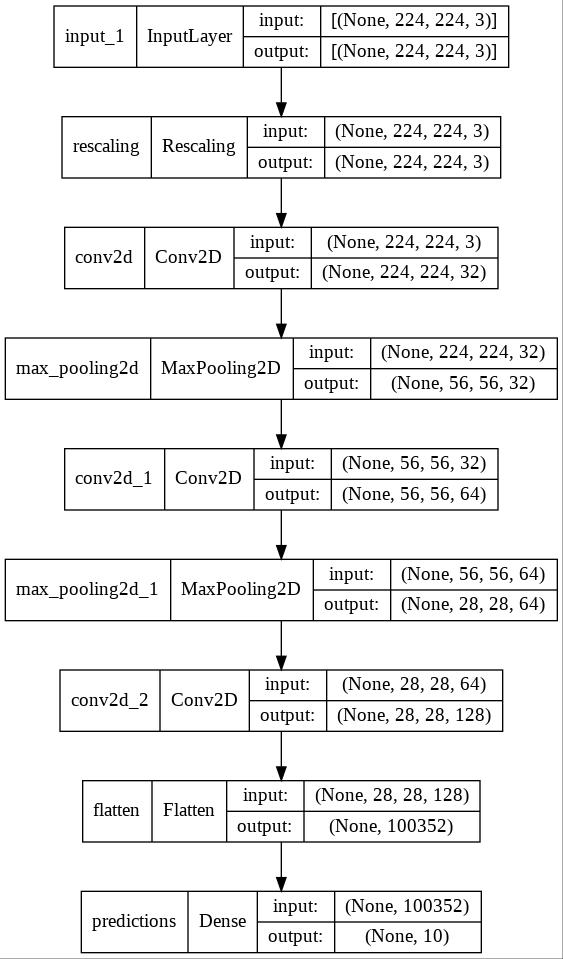
\includegraphics[height=0.6\textwidth]{img/scratch/standardCNN.jpg}
	\caption{Customized Standard CNN Architecture}
	\label{fig:standardCNN}
\end{figure}

\noindent This model is trained using these default hyperparameters:
\begin{itemize}
\item optimizer: \textit{ADAM}
\item dropout rate :0.0
\item learning rate: optimizer's default
\item batch size: 128
\item learning rate decay: none
\end{itemize}

\noindent In particular, we set a large value for batch size both because our main goal is to maximize the accuracy and also (as presented in the Introduction) to face off with the great variability of paintings with very dissimilar style but belonging to the same author. In this way, we increase the probability of a batch to be "complete", thus being representative of this variability.

\noindent The results obtained are the following:

\medskip

\begin{tabular}{ |p{2cm}|p{2cm}|p{2cm}|p{2cm}|p{2cm}|  }
\hline
\multicolumn{5}{|c|}{StandardCNN} \\
\hline
\textbf{Epoch stopped} & \textbf{Validation Accuracy} & \textbf{Testing Accuracy} & \textbf{Validation Loss} & \textbf{Testing Loss} \\
\hline
15 & 0.5730 & ??? & 1,3656 & ???\\
\hline
\end{tabular}

\medskip

\begin{figure}[H]
	\centering
	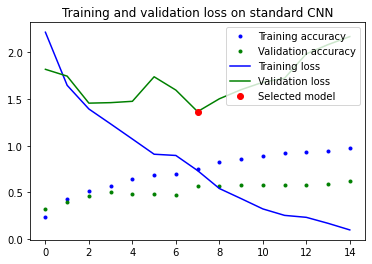
\includegraphics[height=0.45\textwidth]{img/scratch/standardCNN_results.png}
	\caption{Standard CNN: results}
	\label{fig:standardCNN_acc}
\end{figure}
\section{Pre-Trained Models}

\subsection{ResNet50V2}

\subsubsection{Test 1: Classical ResNet50V2 with 50 classes}
On a small dataset, overfitting will be the main issue. Data augmentation is a powerful way to fight overfitting when you’re working with image data.

\subsubsection{Test 2: Completely New Output Layers Architecture}

\subsubsection{Test 3: 1 and 2 with Data Augmentation}

\subsubsection{Test 4: Fine Tuning with One Layer}

\subsubsection{Test 5: Fine Tuning with Two Layers}

\subsubsection{Test 6: Genetic Algorithm for Hyper-parameters and Architecture Optimization}







\subsection{ResNet101V2}

\subsubsection{Test 1: Classical ResNet101V2 with 50 classes}

\subsubsection{Test 2: Completely Newly Output Layers Architecture}

\subsubsection{Test 3: Fine Tuning with One Layer}

\subsubsection{Test 4: Fine Tuning with Two Layers}







\subsection{InceptionV3}

\subsubsection{Test 1: Classical ResNet101V2 with 50 classes}

\subsubsection{Test 2: Completely Newly Output Layers Architecture}

\subsubsection{Test 3: Fine Tuning with One Layer}

\subsubsection{Test 4: Fine Tuning with Two Layers}

\section{Baseline Analysis}
\subsection{Siamese Network}
\subsection{Convolutional Siamese Network}
\section{Ensemble Network}
 Ensembling consists of pooling together the predictions of a set of different models to produce better predictions. Nowadays, in every machine learning competitions, in particular on Kaggle, the winners use very large ensembles of models that inevitably beat any single model, no matter how good, hence we decided to use it also in our project.
 
 
Ensembling relies on the assumption that different well-performing models trained independently are likely to be good for different reasons: each model looks at slightly different aspects of the data to make its predictions, getting part of the “truth” but not all of it\footnote{This can be see in detail in the "data visualization" chapter}. By pooling the perspective of different models together, a far more accurate description of the data can be obtained.

\subsection{Our approach}
In our project we decided to use a simple ensembling approach, which is \textit{average voting}: average voting computes the average of the scores (i.e., softmax output) of the base classifiers and select the class with the highest score.

Although we decided to use this simple approach, even if it is very common, we decided to optimize the choice of models to be used in order to maximize the accuracy obtained on the testset. In fact, all the models described in the chapter "pre-trained models" have been saved as \textit{".keras"} models so that they can be reloaded and used to directly evaluate the testset in the ensemble, so that they do not need to be trained again (thus increasing the speed of test execution).

The main problem was to choose which of these models combined together obtained the best accuracy. Since the number of models was more than 20 a grid search seemed too slow as a method of solving this problem, so we decided to use a genetic algorithm to solve the problem automatically.




\subsubsection{The Ensemble Class}
To perform the ensemble in an orderly fashion, what was done was to create a class called \textit{Ensemble}. The class allows to construct, predict and evaluate in a simple way ensemble networks composed of different models. Here the code:

\begin{python}
class Ensemble:

    def __init__(self, test_images_vgg, test_images_resnet, test_images_inception):
        self.test_images_vgg = test_images_vgg
        self.test_images_resnet = test_images_resnet
        self.test_images_inception = test_images_inception

        # obtain original labels
        self.labels = np.array([])
        for x, y in self.test_images_vgg:
            self.labels = np.concatenate([self.labels, np.argmax(y.numpy(), axis=-1)])

        # create list of models
        self.model_list = []

        base_dir = './models/'
        # VGG16
        for name in vgg16:
            self.model_list.append(ks.models.load_model(base_dir + 'vgg16/' + name))

        # ResNet50
        for name in resnet50:
            self.model_list.append(ks.models.load_model(base_dir + 'resnet50/' + name))

        # ResNet50
        for name in resnet101:
            self.model_list.append(ks.models.load_model(base_dir + 'resnet101/' + name))

        # Inception
        for name in inception:
            self.model_list.append(ks.models.load_model(base_dir + 'inception/' + name))

        # compute all prediction once for all
        self.predictions = []
        for i, model in enumerate(self.model_list):
            if i < len(vgg16):
                self.predictions.append(model.predict(self.test_images_vgg))
            elif i < len(vgg16) + len(resnet50) + len(resnet101):
                self.predictions.append(model.predict(self.test_images_resnet))
            else:
                self.predictions.append(model.predict(self.test_images_inception))

    def predict(self, active_models):
        sum_prediction = None
        start = 0
        count = 0

        if np.sum(active_models) == 0:
            return None

        for start, active_model in enumerate(active_models):
            if active_model == 1:
                sum_prediction = self.predictions[start]
                count += 1
                break

        # additional model selected and added
        for i in range(start + 1, len(self.model_list)):
            if active_models[i] == 0:
                continue
            sum_prediction += self.predictions[i]
            count += 1

        print(count)
        final_preds = 1 / count * sum_prediction
        return np.argmax(final_preds, axis=1)

    def evaluate(self, predictions):
        if predictions == 0:
            return 0

        count = 0
        for i, prediction in enumerate(predictions):
            if int(self.labels[i]) == prediction:
                count += 1
        return count/len(self.labels)

    def predict_and_evaluate(self, active_models):
        return self.evaluate(self.predict(active_models))

    def labels_len(self):
        return len(self.labels)
        
    def models_len(self):
        return len(self.model_list)
\end{python}

The \textit{constructor} takes in input 3 datasets that are equal to each other except for the size of the images, in fact VGG, ResNet and Inception want in input images with size (256,256), (224, 244) and (299,299) respectively: this is done in order to correctly evaluate the models without having errors due to the input data. The constructor also computes the labels of each test sample, loads the models and computes the predictions for each of them, this is done to speed up the execution of the genetic algorithm.

Moving on to discuss the \textit{predict} function, it takes as input an array of length equal to the total number of models consisting of zeros or ones. The array indicates the models to be used: in the same position where a one is present the corresponding model inside {model\_list} must be used.

As for the \textit{evaluate} function, it takes an array of predictions and returns the accuracy, calculated as the number of correct predictions over the total number of test samples.

\subsubsection{Genetic Algorithm Workflow}
Following the guidelines in Section 2.6, we need to decide how to develop the different components and decide on the hyperparameters in order to define the flow of the genetic algorithm.

\paragraph{Genotype}
In our specific case, our chromosomes are binary encoded and each gene represents a different model. Hence, we have individuals made of a number of genes equal to the number of different models that we have.

\begin{python}
# create an operator that randomly returns 0 or 1
toolbox.register('zeroOrOne', random.randint, 0, 1)

# define a single objective, maximizing fitness strategy:
creator.create('FitnessMax', base.Fitness, weights=(1.0,))

# create the Individual class based on list:
creator.create('Individual', list, fitness=creator.FitnessMax)

# create the individual operator to fill up an Individual instance:
toolbox.register('individualCreator', tools.initRepeat, creator.Individual, toolbox.zeroOrOne, INDIVIDUAL_LENGTH)
\end{python}

\paragraph{Population}
The population is composed of 100 individuals, we decided to keep a high number of individuals in order to have more chances to have more different individuals and therefore to have different starting points in order to converge better to the optimal solution. Although the number of individuals may seem very high, we decided to increase the speed of the computation of the prediction simply by calculating once and for all the values of the predictions for each classifier at the creation of the Ensemble class, and save them in memory for later use without having to recompute them.

\begin{python}
toolbox.register('populationCreator', tools.initRepeat, list, toolbox.individualCreator)
\end{python}

\paragraph{Fitness Function}
The fitness function is the accuracy obtained through the \textit{predict\_and\_evaluate} function of the Ensemble class. It was registered in the \textit{toolbox} as follows:

\begin{python}
def ensembleAccuracy(individual):
    return ensemble.predict_and_evaluate(individual)

toolbox.register('evaluate', ensembleAccuracy)
\end{python}

\paragraph{Selection Algorithm}
The selection algorithm used in this case is \textit{tournament selection}. In each round of the tournament selection method, two individuals are randomly picked from the population, and the one with the highest fitness score wins and gets selected. We decided to select only five individuals since our population is small and selecting more could cause an abuse in exploitation.

\begin{python}
# Tournament selection with tournament size of 5:
toolbox.register("select", tools.selTournament, tournsize=5)
\end{python}


\paragraph{Crossover Algorithm}
As crossover algorithm we decided to use the \textit{two-point crossover}. In the two-point crossover method, two crossover points on the chromosomes of both parents are selected randomly. The genes residing between these points are swapped between the two parent chromosomes.

The following diagram demonstrates a two-point crossover carried out on a pair of binary chromosomes, with the first crossover point located between the third and fourth genes, and the other between the seventh and eighth genes:

\begin{figure}[H]
	\centering
	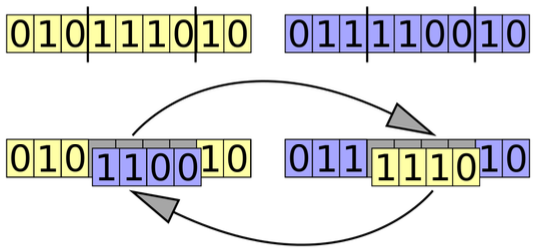
\includegraphics[width=0.4\textwidth]{img/twopointcross.png}
	\caption{Two point crossover example.}
	\label{fig:twopointcross}
\end{figure}

The code for that is:
\begin{python}
toolbox.register("mate", tools.cxTwoPoint)
\end{python}

\paragraph{Mutation Algorithm}
As mutation algorithm we decided to use the \textit{Multiple Flip bit mutation}. When applying the flip bit mutation to a binary chromosome, one gene is randomly selected and its value is flipped (complemented), as shown in the following diagram:

\begin{figure}[H]
	\centering
	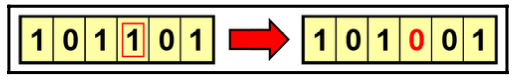
\includegraphics[width=0.4\textwidth]{img/flipbit.png}
	\caption{Flip bit mutation example.}
	\label{fig:flipbit}
\end{figure}

This can be extended to several random genes being flipped instead of just one, obtaining the multiple flip bit mutation that we use.
The code for that is:
\begin{python}
toolbox.register("mutate", tools.mutFlipBit, indpb=1.0/INDIVIDUAL_LENGTH)
\end{python}


\paragraph{Elitism}
We set the number of individuals for the elitism mechanism to 5. This value has been chosen in consideration of the fact that the number of individuals is 100, not very high, and that an individual is composed of little more than twenty genes: if we chose a higher value for the hall of fame, what could happen is that we could not exploit much the global search carried out by the exploration because we would end up with very similar chromosomes; therefore, in order not to risk bad results, we chose to use this conservative approach and limit the number to these few.

\paragraph{GA Flow}
The first thing to do is to define the initial population, this is easily done by the following line of code:

\begin{python}
population  = toolbox.populationCreator(n=POPULATION_SIZE)
\end{python}

After that, we created a statistical object. This object has served to have a report of the flow of the genetic algorithm, allowing us to save for each generation the maximum and average fitness values obtained, so that we can show them once the generations are over.

\begin{python}
stats = tools.Statistics(lambda ind: ind.fitness.values)
stats.register("max", np.max)
stats.register("avg", np.mean)
\end{python}

Then, the last object we need to create for the \textit{eaSimple} is the \textbf{HallOfFame}, which can be done through the following line of code:

\begin{python}
hof = tools.HallOfFame(HALL_OF_FAME_SIZE)
\end{python}

The main flow is done using the \textit{eaSimple} in the way as follow:

\begin{python}
population, logbook = eaSimpleWithElitism(population,
								  toolbox,
								  cxpb=P_CROSSOVER,
								  mutpb=P_MUTATION,
								  ngen=MAX_GENERATIONS,
								  stats=stats,
								  halloffame=hof,
								  verbose=True)
\end{python}

Where the P\_CROSSOVER is equal to 0.9, P\_MUTATION 0.1.\footnote{Value suggested by the book ”Hands on Genetic Algorithms with Python” by Eyal Wirsansky, also the other values of probabilities are taken by the suggestions of the book}


\end{document}